\documentclass[a4paper,landscape]{article}

\usepackage[landscape,top=0cm,left=0cm,bottom=0cm,right=0cm]{geometry}
\usepackage{tikz}
\usepackage{background}
\usepackage{blindtext}
\usetikzlibrary{matrix, shapes.misc, calc}

\pagestyle{empty}
\setlength{\parindent}{0cm}
\backgroundsetup{scale = 1, angle = 0, opacity = 1, color=black, contents = {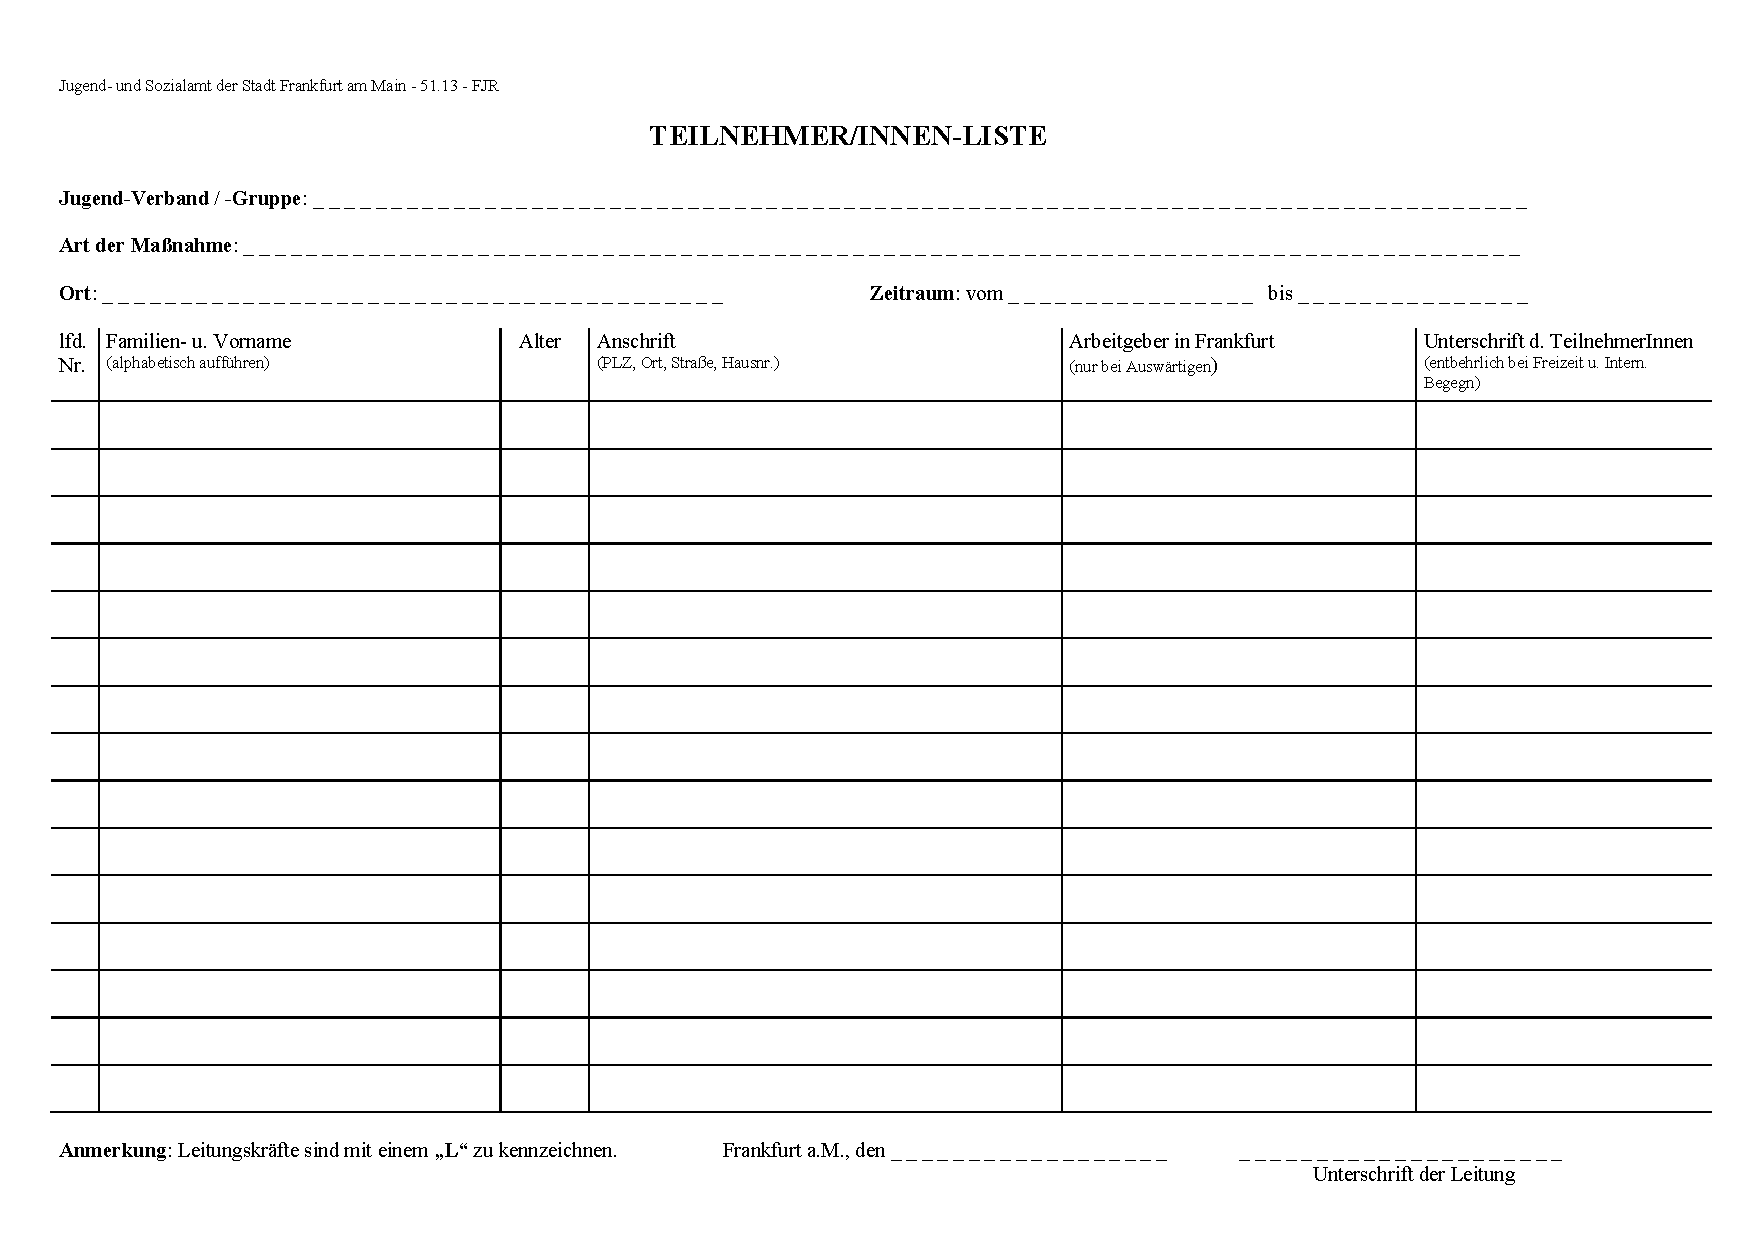
\includegraphics[width = \paperwidth, height = \paperheight] {city-frankfurt-main.pdf}}}

\begin{document}
    \noindent \sffamily

    @foreach($members as $i => $chunk)
        \begin{tikzpicture}[remember picture,overlay,yscale=-1]
            \node[anchor=base west, text width=205.3mm] at (52.9mm,31.0mm) {\bfseries{\large{<<<!!$fromName!!>>>}}};   %Feld: Jugendverband/-Gruppe
            \node[anchor=base west, text width=215.9mm] at (41.3mm,38.8mm) {\bfseries{\large{<<<!!$eventName!!>>>}}};   %Feld: Art der Maßnahme
            \node[anchor=base west, text width=104.8mm] at (17.5mm,47.0mm) {\bfseries{\large{<<<!!$zipLocation!!>>>, <<<!!$countryName!!>>>}}};
            \node[anchor=base west, text width=41.3mm, align=center] at (170.7mm,47.0mm) {\bfseries{\large{<<<!!$niceDateFrom()!!>>>}}};
            \node[anchor=base west, text width=38.4mm, align=center] at (219.9mm,47.0mm) {\bfseries{\large{<<<!!$niceDateUntil()!!>>>}}};

            @foreach($chunk as $j => $member)
                \node[anchor=base, text width=4mm, align=center] at ($(8.0mm, 69.0mm + 8.05mm * <<<$j%15>>>)$) {<<<$member->isLeader ? 'L' : ''>>>};
                \node[anchor=base, text width=6mm, align=center] at ($(13.0mm, 69.0mm + 8.05mm * <<<$j%15>>>)$) {<<<$j+1>>>};
                \node[anchor=base, text width=67.5mm, align=center] at ($(50.65mm, 69.0mm + 8.05mm * <<<$j%15>>>)$) {<<<$member->separatedName()>>>};
                \node[anchor=base, text width=14.6mm, align=center] at ($(92.2mm, 69.0mm + 8.05mm * <<<$j%15>>>)$) {<<<$member->age()>>>};
                \node[anchor=base, text width=79.4mm, align=center] at ($(139.7mm, 69.0mm + 8.05mm * <<<$j%15>>>)$) {<<<$member->fullAddress()>>>};
            @endforeach

            \node[anchor=base, text width=23.0mm, align=center] at (278.2mm,196.1mm) {Seite <<<!!$i + 1!!>>> von <<<!!$pages!!>>>};

        \end{tikzpicture}

        \pagebreak

    @endforeach
\end{document}

